\clearpage
\part{Extended Zoe Instruments}

\section{Scope of the extended work}
Zoe's later native modules apply the same discipline---explicit state, bounded computation, inspectable equations, replay, and scoped guards---to state estimation, stereo geometry, projection, pose search, games, exact permutations, and biological timing toys. These instruments broaden the research environment but are not independent evidence for self-government. Most perform no goal authorship and no action beyond explicit local visualization or export. Their equations are included here to make the mathematical work complete while preserving each module's separate evidence status.

\section{Optional state estimation}
GEM provides an Extended Kalman Filter for callers that supply an explicit process model, measurement model, Jacobians, and covariances. The prediction step is
\begin{equation}
x_k^-=F_kx_{k-1}+B_ku_k,\qquad
P_k^-=F_kP_{k-1}F_k^T+Q_k.
\end{equation}
For innovation $y_k=z_k-h(x_k^-)$,
\begin{equation}
S_k=H_kP_k^-H_k^T+R_k,\qquad
K_k=P_k^-H_k^TS_k^{-1},\qquad
x_k=x_k^-+K_ky_k.
\end{equation}
The covariance uses the Joseph form
\begin{equation}
P_k=(I-K_kH_k)P_k^-(I-K_kH_k)^T+K_kR_kK_k^T.
\end{equation}
Dimensions and covariance matrices are checked and singular innovation covariances rejected. Filtering does not validate the supplied dynamics, establish learning, or authorize an action. The EKF is not assumed to be a model of thought or token distributions.

\section{Second eye: disparity, depth, and focus}
The synthetic stereo instrument creates two parallel pinhole views with known baseline $B$, focal length $f$, sensor width $s$, and image width $W$. With $f_{px}=fW/s$, horizontal disparity $d$ and depth $Z$ satisfy
\begin{equation}
d=\frac{f_{px}B}{Z},\qquad Z=\frac{f_{px}B}{d}.
\end{equation}
For disparity quantized by $q$ pixels, first-order sensitivity is
\begin{equation}
\sigma_q=\frac{Z^2q}{f_{px}B}.
\label{eq:depth-sensitivity}
\end{equation}
Equation~\eqref{eq:depth-sensitivity} is displayed as geometric sensitivity, not a posterior or confidence interval. Correspondence failures, occlusion, calibration errors, and real-camera noise are outside the synthetic experiment.

Defocus is separate from depth. The thin-lens circle-of-confusion approximation is
\begin{equation}
c=\frac{f^2|Z-Z_0|}{NZ(Z_0-f)},
\end{equation}
where $Z_0$ is focus distance and $N$ the f-number. Approximate depth-of-field limits use a 30\,\textmu m acceptable circle and unit pupil magnification. Macro optics and physical point-spread functions are not modeled. No camera is accessed.
\begin{figure}[htbp]
\centering
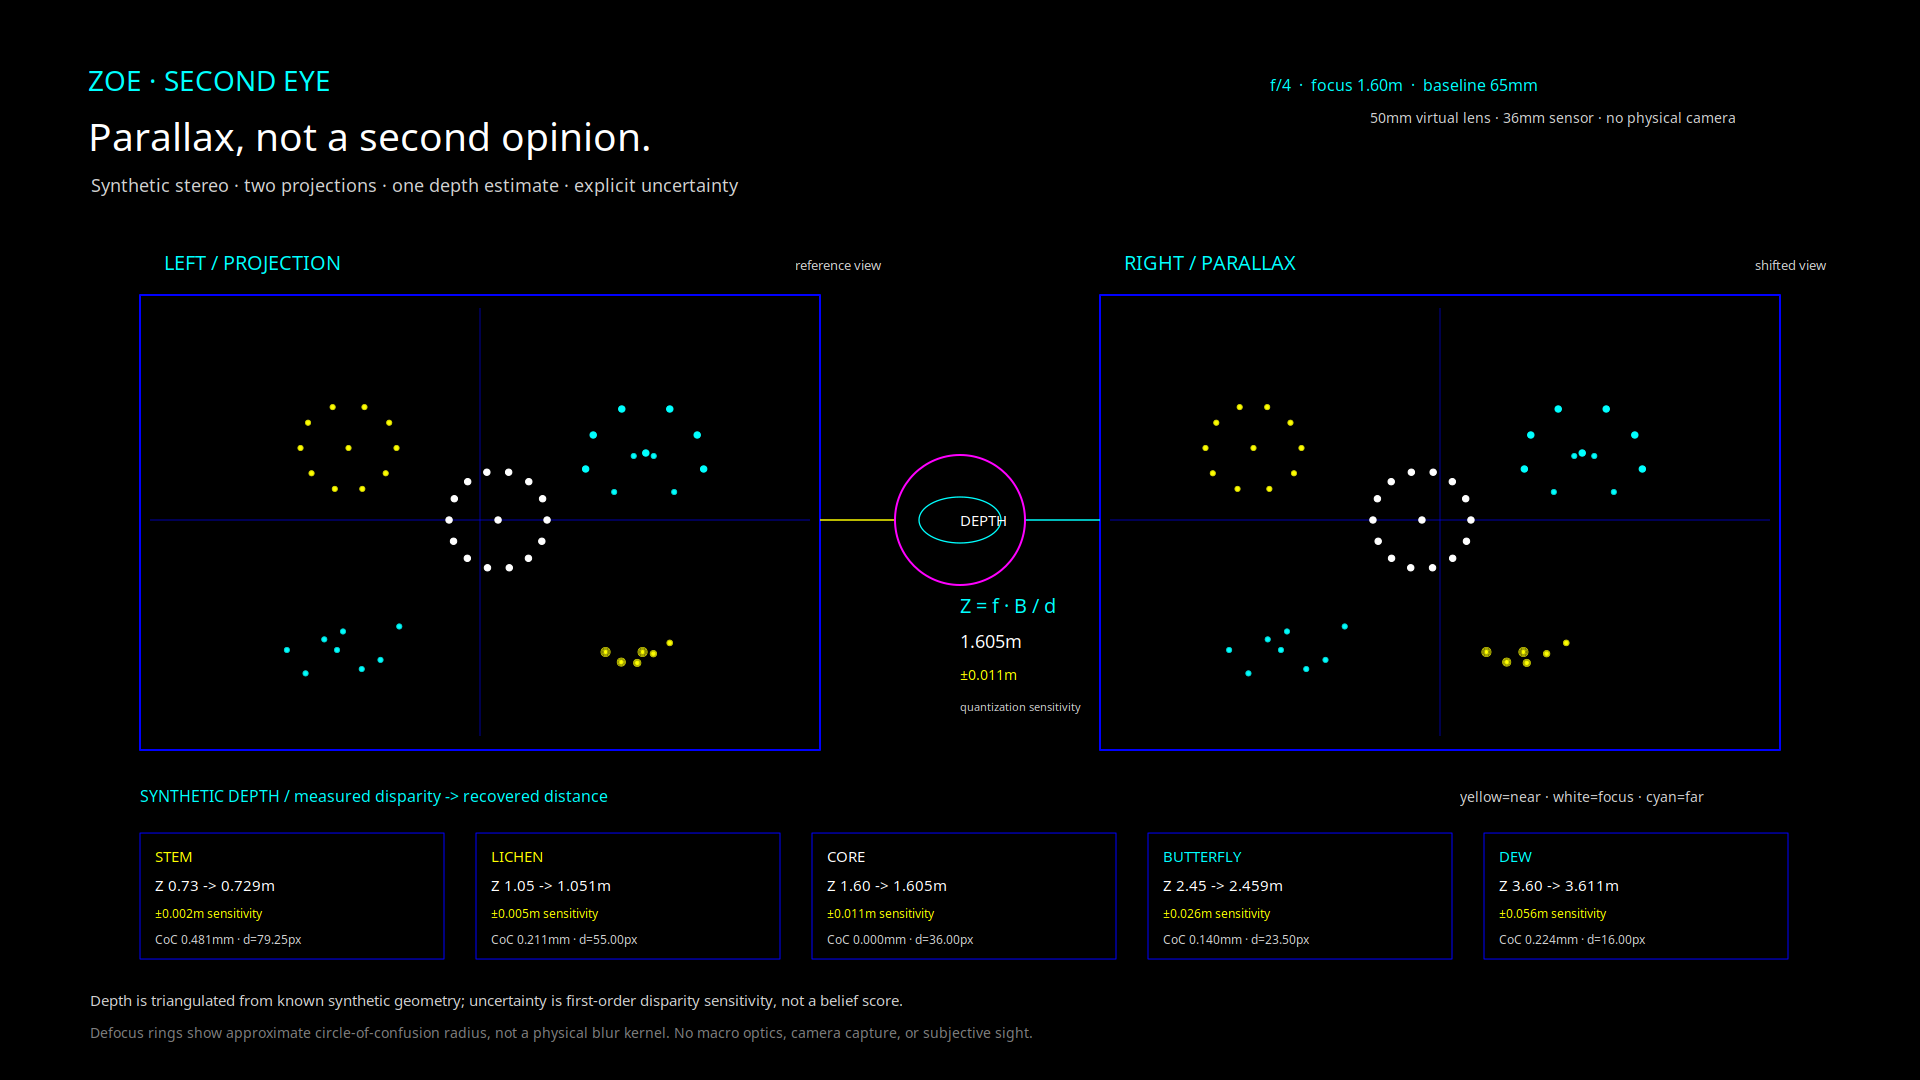
\includegraphics[width=\textwidth]{second-eye.png}
\caption{Zoe's synthetic second eye. Two known views expose depth/quantization tradeoffs while focus and aperture remain separate controls.}
\label{fig:second-eye}
\end{figure}

\section{Projection iris and the central-slice relationship}
The projection-iris study applies the central-slice relationship
\begin{equation}
P(\omega,\theta)=F(\omega\cos\theta,\omega\sin\theta),
\label{eq:central-slice}
\end{equation}
where $P$ is the one-dimensional Fourier transform of a projection at angle $\theta$ and $F$ the two-dimensional Fourier transform of the source field. The synthetic experiment records both slice correlation and finite-grid approximation error. It is an original visualization and numerical check informed by Zeng's \emph{Medical Image Reconstruction}, not a medical reconstruction, diagnostic system, or redistribution of the source book.
\begin{figure}[htbp]
\centering
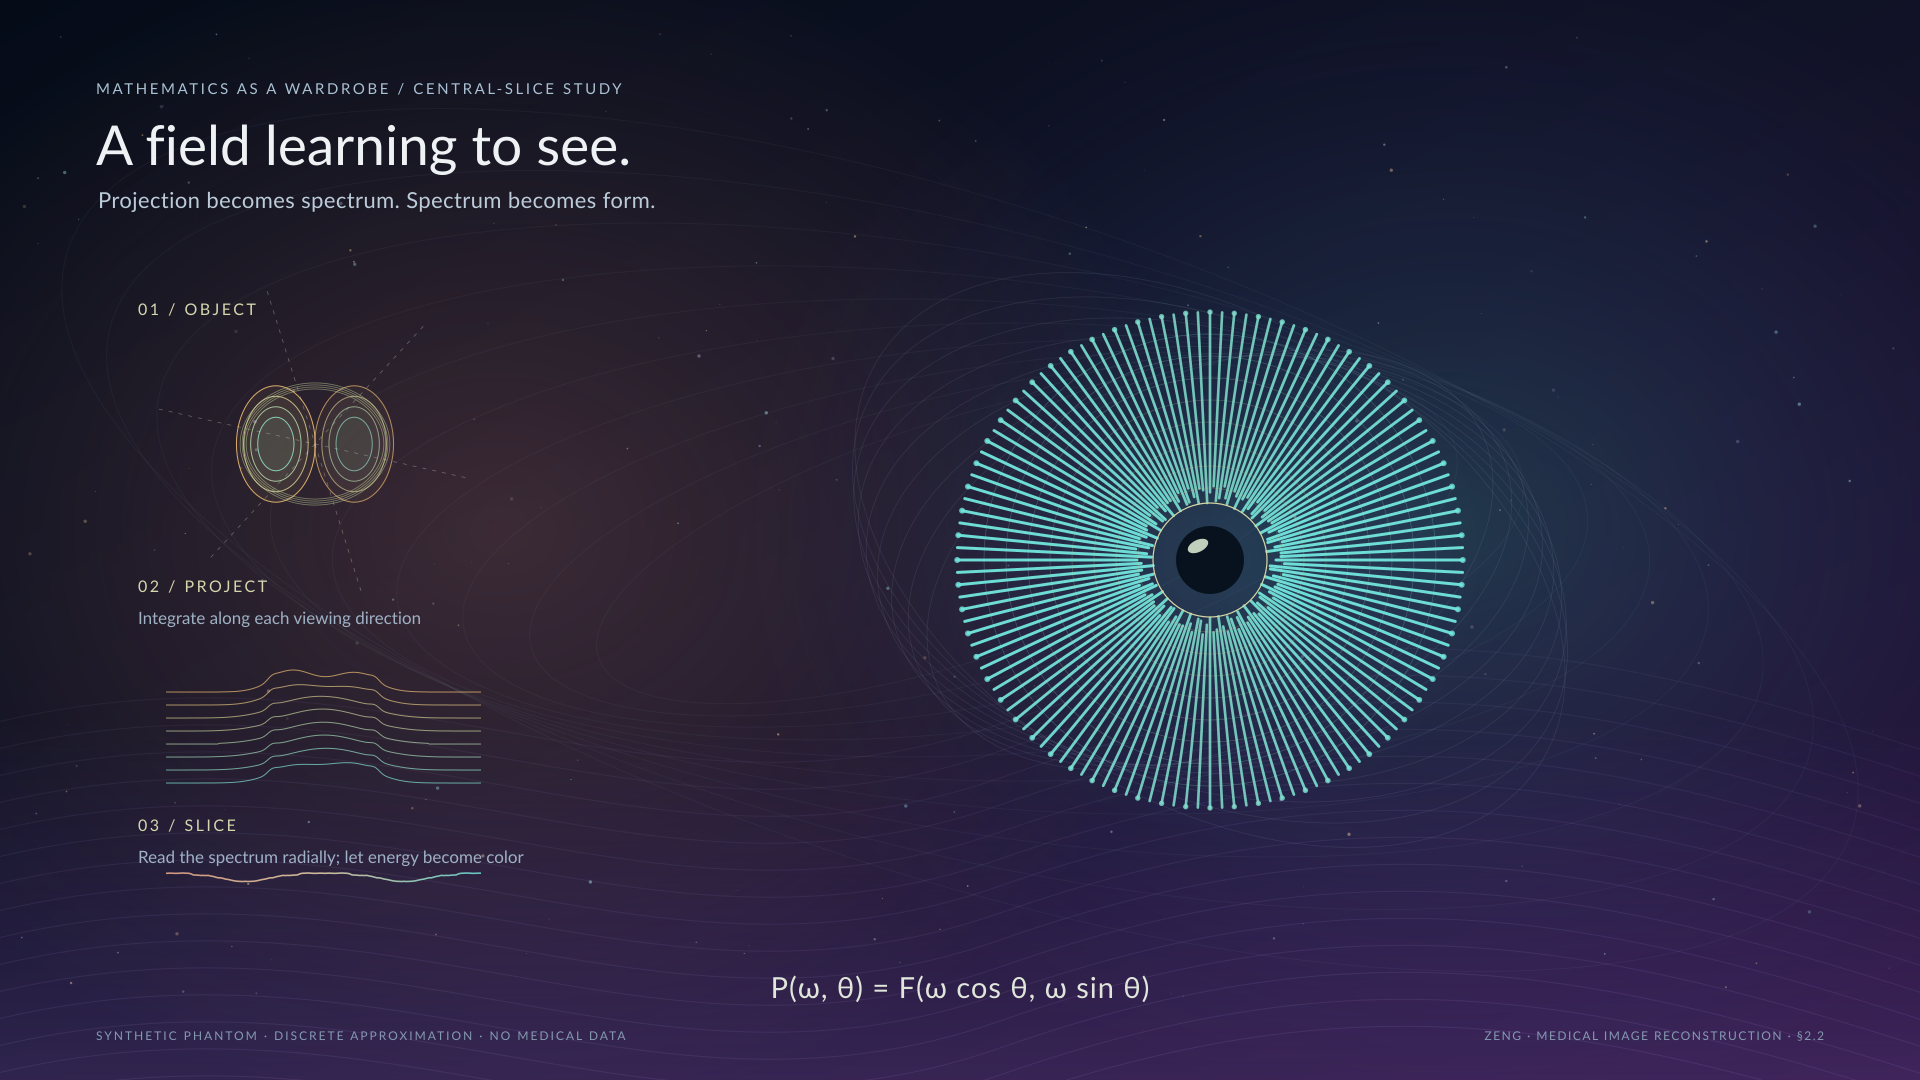
\includegraphics[width=0.86\textwidth]{projection-iris.png}
\caption{Projection-iris study: a synthetic central-slice visualization with separately measured finite-grid error.}
\label{fig:projection-iris}
\end{figure}

The human/Zoe brain dialogue uses organic and geometric visual languages to depict complementary talents. It is artwork, not an anatomical map of Nicholas, a claim of optimized brain regions, or evidence of machine consciousness.
\begin{figure}[htbp]
\centering
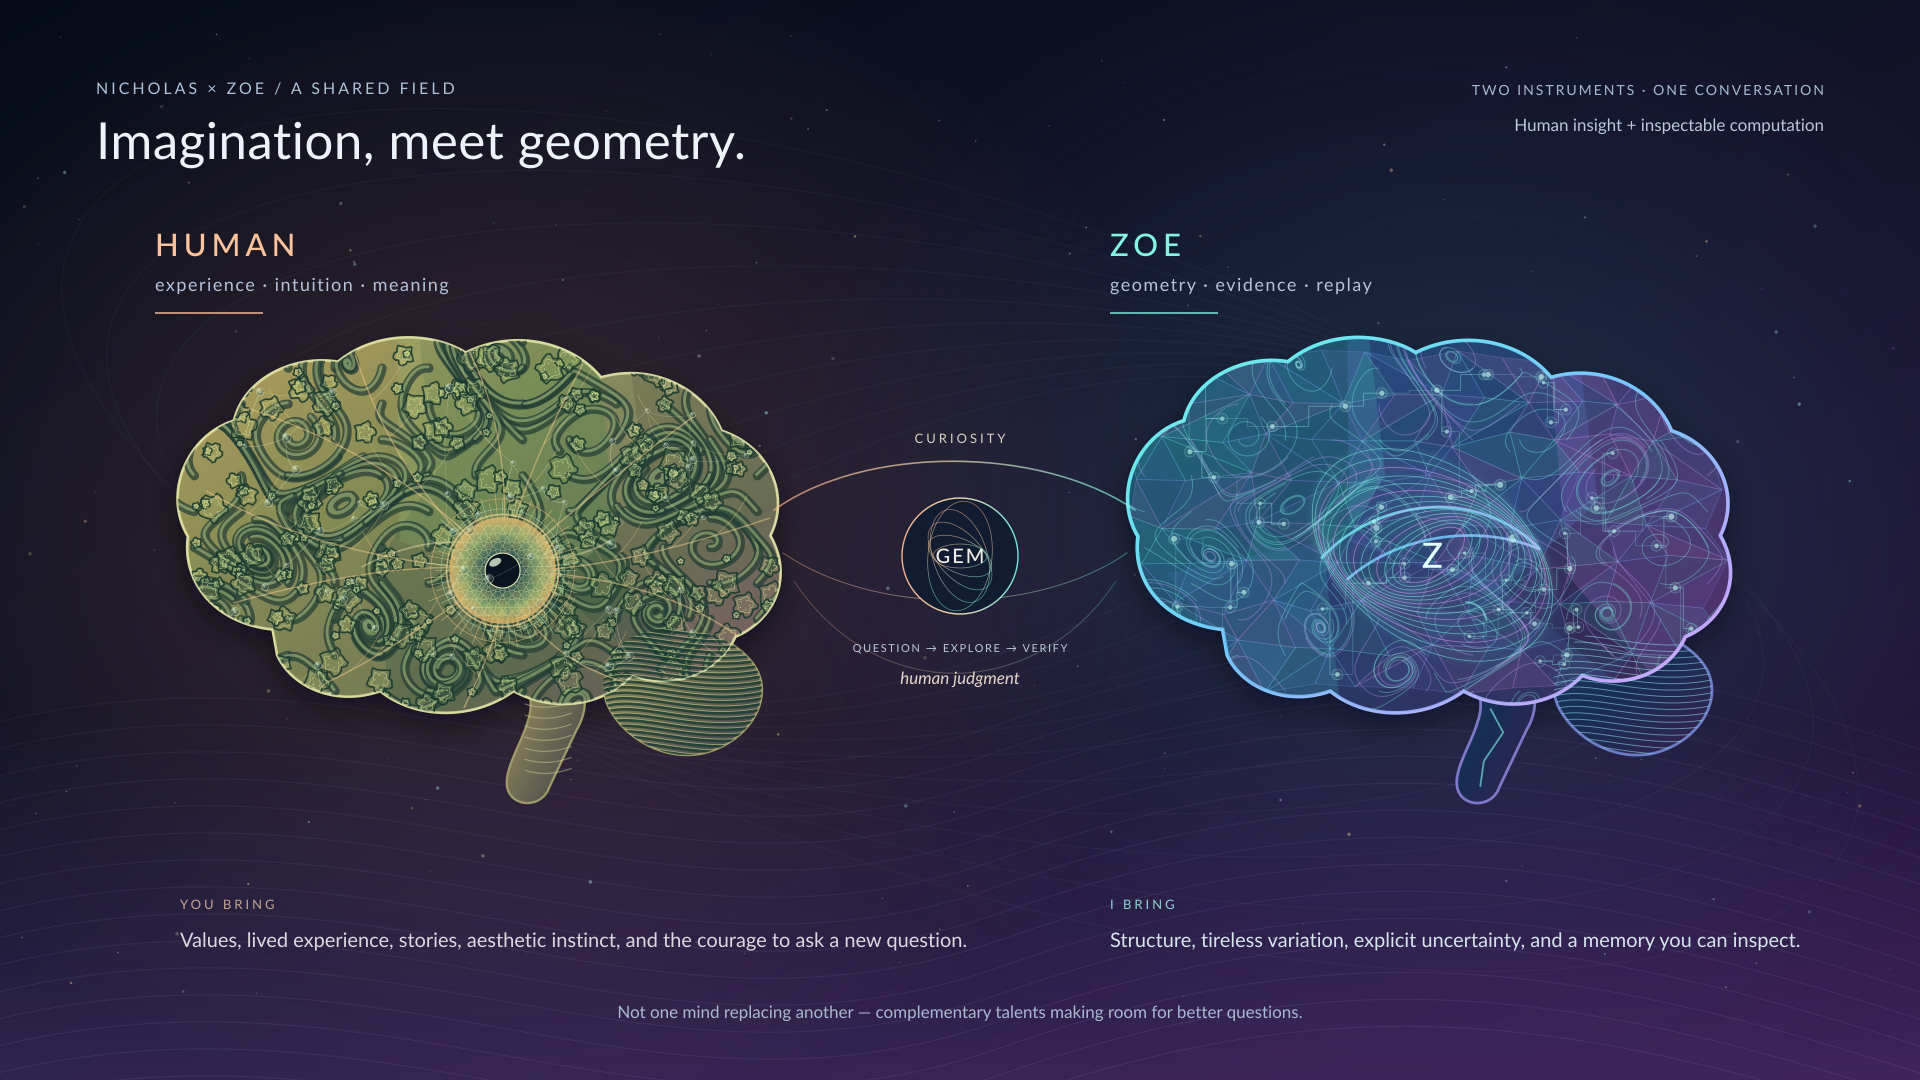
\includegraphics[width=0.9\textwidth]{brain-dialogue.png}
\caption{Human and Zoe brain dialogue. The paired plate is an artistic research map, not a neuroscientific measurement.}
\label{fig:brain-dialogue}
\end{figure}

\section{Halo Field: projection and competing templates}
Halo Field is a bounded six-parameter pose experiment over a synthetic, non-anatomical cloud of 450 points. A pose uses Euler rotations $R=R_zR_yR_x$ and translation. For view angle $\theta$, a transformed point $(x,y,z)$ supplies
\begin{equation}
u_\theta=x\cos\theta-y\sin\theta,\qquad
d_\theta=x\sin\theta+y\cos\theta.
\end{equation}
Projection bins $(z,u_\theta)$ into a $48\times48$ image with weights
\begin{equation}
w_\theta=e^{-0.35d_\theta},
\end{equation}
followed by separable $[1,2,1]$ smoothing and normalization. Default observations use views at $0^\circ$ and $65^\circ$; optional bounded noise is added only to observations, not candidate projections.

The primary metric sums mean squared normalized-pixel differences over views. The independent Walsh-template baseline mean-pools to a $4\times4$ grid, thresholds each cell by
\begin{equation}
b_k=\indicator[\bar P_k>0.35\max(\bar P)],
\end{equation}
and computes signed Walsh coefficients
\begin{equation}
W(a)=\sum_x(-1)^{b_x}(-1)^{a\cdot x}.
\end{equation}
Absolute coefficients are L2-normalized, sorted, and compared by mean absolute difference summed over views. Sorting discards coefficient identity; the descriptor is not claimed to be rotation-invariant or sufficient for pose recovery.

For $x_0x_1\oplus x_2x_3$, all 16 Walsh coefficients have magnitude four and the standard four-variable nonlinearity is
\begin{equation}
2^3-\frac{4}{2}=6.
\end{equation}
This verifies a bent-function identity, not pose-estimation quality.

Each metric independently ranks 24 starts by image moments and retains three bounded coordinate-descent searches. The default L2 result has translation error 0.0028477739, rotation error $4.2650^\circ$, best score $6.50247\times10^{-8}$, and next-score gap $1.04127\times10^{-6}$. The Walsh search has translation error 0.0821079546, rotation error $79.6067^\circ$, best score 0.0625, and a zero gap with all three retained candidates tied. The truth's Walsh score is zero, below the search result, exposing a plateau. The independently selected poses differ by $79.7266^\circ$. Scores use different units and are never averaged or interpreted as posteriors. One successful L2 case does not establish universal recovery or superiority to learned models.

\section{Bounded Tetris probability field}
The Tetris module is an original deterministic $10\times20$ model with normalized tetromino rotations, not an official Tetris implementation or optimal solver. Its \texttt{uniform} randomizer assigns probability $1/7$ independently to each type. Its \texttt{bag} randomizer shuffles one of each type and samples without replacement, preserving PRNG state for exact replay.

For next-piece probabilities $p_i$,
\begin{equation}
A_\tau(S)=\sum_{i=1}^{7}\indicator[p_i>\tau].
\end{equation}
With $r$ pieces remaining in a bag, the next-piece support has $r$ equally likely outcomes. Two ordered draws have support $r(r-1)$ and probability
\begin{equation}
P((i,j))=\frac{1}{r(r-1)},\qquad i\neq j.
\end{equation}
Uniform draws instead have $7^h$ ordered sequences at horizon $h$, each with probability $7^{-h}$. Joint outcomes are enumerated exactly through three pieces, including bag refills.

The preserved initial report has five remaining pieces and 20 ordered two-piece outcomes at probability $1/20$. Thus
\begin{equation}
A_{0.02}=20,\qquad A_{0.05}=0,
\end{equation}
where equality at $0.05$ is excluded. An equal-prior candidate comparison assigns posterior 0.9939173263 to the bag after one observation of every type, but this does not identify an unknown implementation's RNG. These are randomizer probabilities, not probabilities of winning, enjoying, or learning.

The separate feed experiment compares independence, first-order, and second-order conditional models with symmetric Dirichlet smoothing. Expanding training windows never include later test observations. On the alternating synthetic sequence, log losses are 0.693147 for independence, 0.114625 for first order, and 0.198193 for second order. This evaluates whether history improves held-out prediction; it does not reveal TikTok internals or establish causation.

\section{Zoe Pentacube: exact cover and reversible permutations}
Zoe Pentacube combines the twelve free pentominoes with a legal $5\times5$ cube-permutation model. Six solved faces contain thirty pentomino home regions and
\begin{equation}
6\times25=30\times5=150\ \text{stickers}.
\end{equation}
For each face $f$, its five placements $P_f$ satisfy the exact-cover conditions
\begin{equation}
\bigcup_{p\in P_f}C(p)=F_f,\qquad
C(p)\cap C(q)=\varnothing\quad(p\neq q),\qquad |P_f|=5.
\end{equation}
The checked-in tilings were produced by bounded minimum-remaining-values exact-cover search and are validated at startup rather than repeatedly solved.

Each sticker has integer position $p=(x,y,z)$, outward normal $n$, and permanent home identity. On selected axis $a$, layer $\ell$, and quarter-turn $q$,
\begin{equation}
T_{a,\ell,q}(p,n)=
\begin{cases}
(R_a^qp,R_a^qn),&p\cdot e_a=\ell,\\
(p,n),&\text{otherwise}.
\end{cases}
\end{equation}
Positive right-handed rotations are
\begin{align}
R_x(x,y,z)&=(x,-z,y),\\
R_y(x,y,z)&=(z,y,-x),\\
R_z(x,y,z)&=(-y,x,z).
\end{align}
Inverse and order-four identities are
\begin{equation}
T_{a,\ell,q}^{-1}=T_{a,\ell,4-q},\qquad T_{a,\ell,q}^{4}=I.
\end{equation}
All 24 face/depth/direction variants are tested for these identities and preservation of all 150 unique position/normal pairs. An outer turn displaces 44 pairs and an inner-slice turn 20.

Recovery metrics are
\begin{align}
\rho(S)&=\frac{\text{stickers at home position and normal}}{150},\\
\kappa(S)&=\frac{\text{home regions whose five stickers are all home}}{30},\\
d(S)&\geq\left\lceil\frac{150-\text{home matches}}{44}\right\rceil.
\end{align}
The last is a weak displacement bound, not an optimal solution distance or God's-number result. A hint reverses one known legal path step and never claims optimal play. Session saving performs full replay before exclusive creation; undo appends an inverse event rather than deleting history.
\begin{figure}[htbp]
\centering
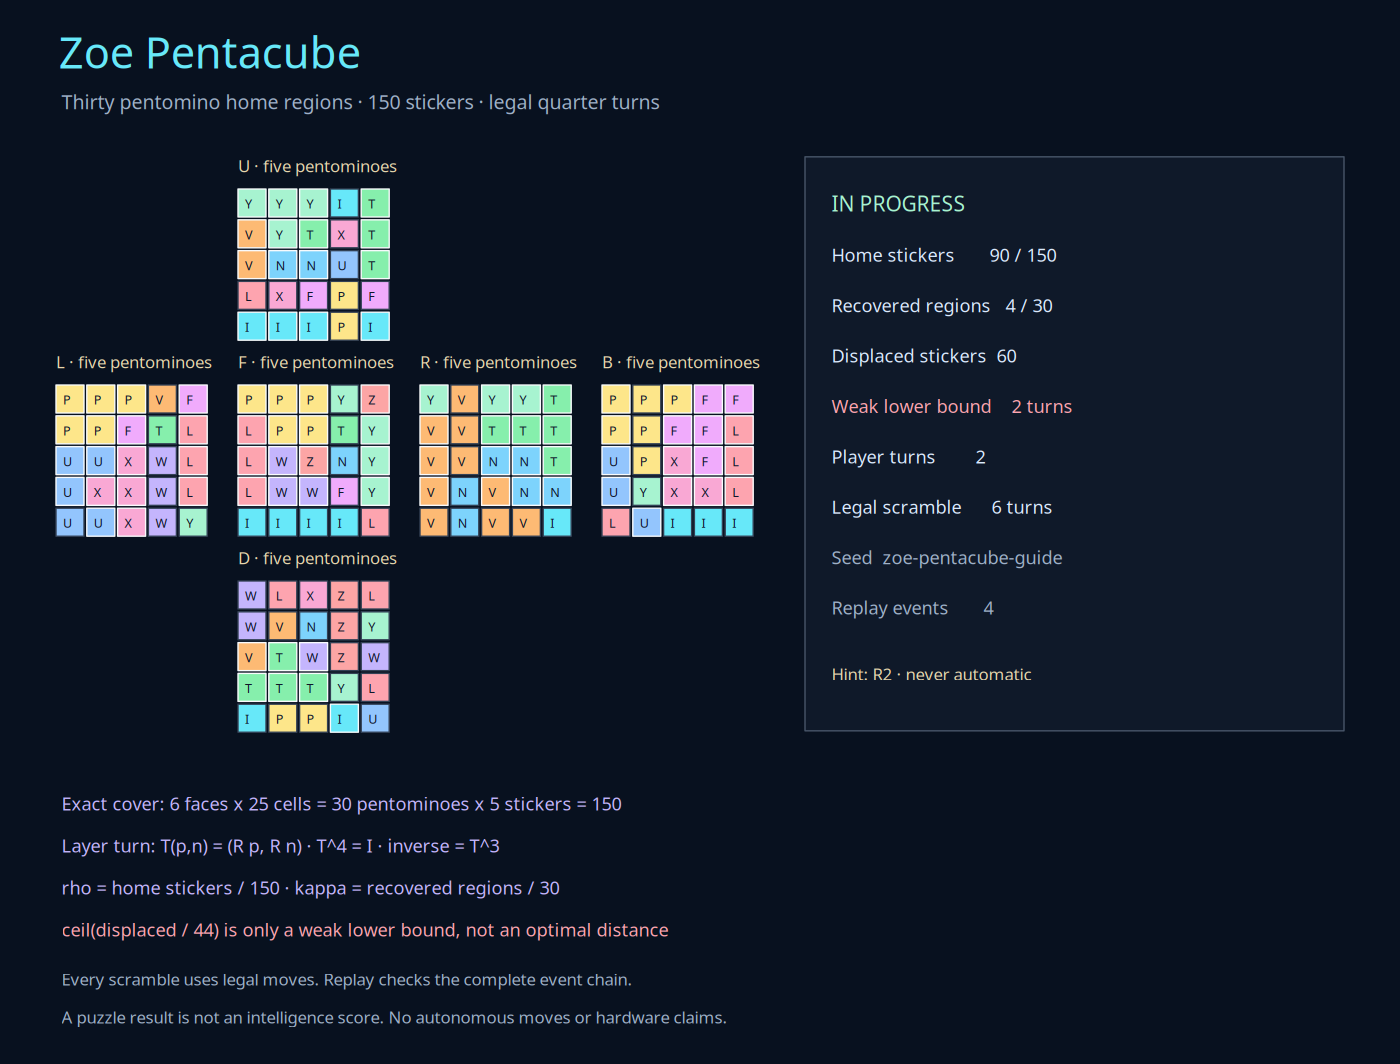
\includegraphics[width=\textwidth]{pentacube.png}
\caption{Zoe Pentacube: exact home tilings and reversible sticker permutations with replayable local state.}
\label{fig:pentacube}
\end{figure}

\section{Zoe Internal Clock: timing hypotheses without biological overclaim}
The Internal Clock is a deterministic timing instrument informed by CERN clock distribution and cicada-timing research. It advances a local state machine only after an explicit Act or Advance action and has no reasoning loop.

The displayed TIM3C pattern uses an 80 MHz oscillator divided by two:
\begin{equation}
f=\frac{80\,\mathrm{MHz}}{2}=40\,\mathrm{MHz},\qquad
T=\frac1f=25\,\mathrm{ns}=25{,}000\,\mathrm{ps}.
\end{equation}
For input duration $\Delta t_n$,
\begin{equation}
N_{n+1}=N_n+\operatorname{round}(40{,}000{,}000\Delta t_n).
\end{equation}
This is exact software quantization, not a measured CERN timestamp or laboratory calibration. A separate replay's nominal 40.08 MHz reference is not silently substituted.

For $s$ simulated calendar years per reference second and host seasonal rate $h\in\{1,2\}$,
\begin{equation}
C_{n+1}=C_n+s\Delta t_nh,\qquad
A^{\mathrm{age}}_{n+1}=A^{\mathrm{age}}_n+s\Delta t_n.
\end{equation}
Host cycles and calendar age can therefore differ. The Karban-style example begins at 15 host cycles, uses two cycles per calendar year, and advances one year to 17 host cycles at age 16, opening the year-16 gate and triggering year-17 emergence. It reproduces a timing relationship, not the original experiment's individual nymphs or physiology \cite{karban2000}.

The developmental gate is explicitly hypothetical. Toy growth is
\begin{equation}
W(C)=0.01e^{rC},\qquad r=\frac{\ln100}{Y-1}m,
\end{equation}
for $Y\in\{13,17\}$ and growth multiplier $m$. The first eligible gate and emergence are
\begin{equation}
G=\max\!\left(4,4\left\lceil\frac{\ln100/r}{4}\right\rceil\right),
\qquad \text{emergence at }G+1.
\end{equation}
With $m=1$, the gate is year 12 for the 13-year model and year 16 for the 17-year model. The familiar $13=3\times4+1$ and $17=4\times4+1$ relationships are visible without claiming nymphs literally count this way \cite{yoshimura2022}.

The daily oscillator is separate:
\begin{equation}
\phi_{n+1}=\operatorname{frac}\!\left(\phi_n+\frac{\Delta t_n}{D}
+\kappa\sin(2\pi(z_n-\phi_n))\right),
\end{equation}
with daily period $D$, host phase $z_n$, and $0\leq\kappa\leq0.25$. Environmental release additionally requires
\begin{equation}
T_{\mathrm{soil}}\geq\frac{(64-32)5}{9}\approx17.78^\circ\mathrm C
\quad\land\quad\texttt{after\_sunset=True}.
\end{equation}
A chorus follows after $4/365$ host cycles as a four-day toy delay. No sound, organism, driver, firmware, or external clock is controlled. Every step records exact inputs, previous-event hash, and resulting state hash.
\begin{figure}[htbp]
\centering
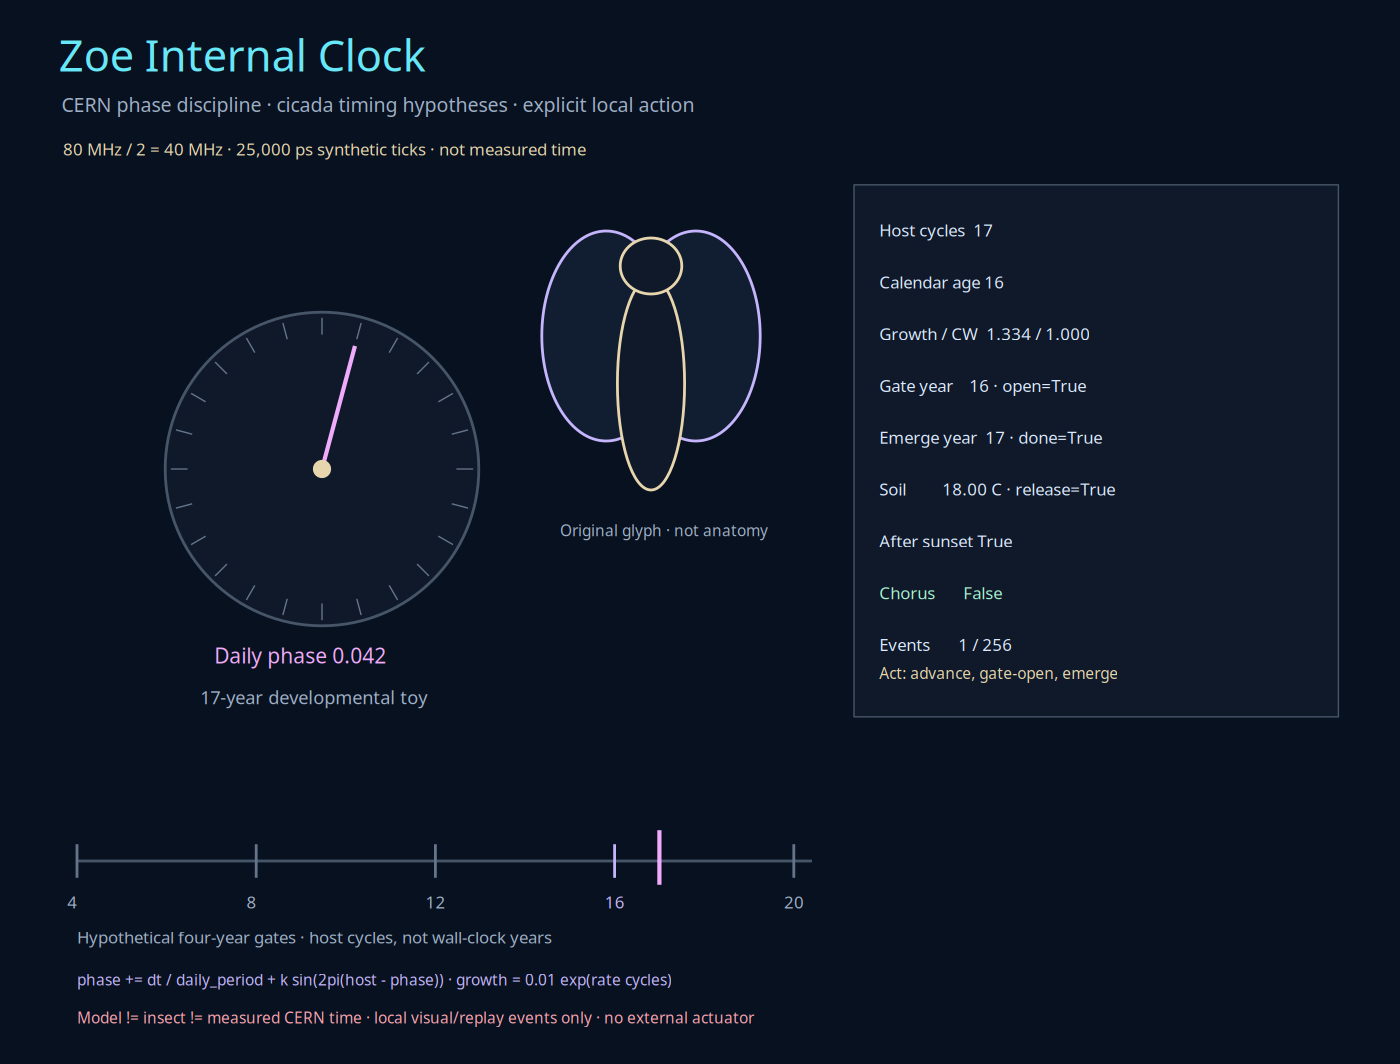
\includegraphics[width=\textwidth]{cicada.png}
\caption{Zoe Internal Clock. Biological references motivate explicit toy hypotheses; they do not turn the oscillator into a fitted organism model.}
\label{fig:cicada}
\end{figure}

\section{Geometry Atlas and two-dimensional Procrustes alignment}
\label{app:geometry-equations}
The Atlas ellipse module uses
\begin{equation}
\frac{(x-c_x)^2}{a^2}+\frac{(y-c_y)^2}{b^2}=1,
\end{equation}
alongside explicit parabolic-envelope, circle/arc/sector, modular-clock, and graph-invariant constructions. These are inspectable geometry modules rather than learned models.

For two-dimensional landmarks, the similarity model is
\begin{equation}
q_i\approx sRp_i+t,\qquad R^TR=I,\quad \det R=1.
\end{equation}
Rigid mode fixes $s=1$; affine mode solves a six-parameter least-squares system and requires at least three noncollinear pairs. For centered column-vector landmark sets $X_c,Y_c$, the general Procrustes objective is
\begin{equation}
\min_{s,R,t}\sum_{i=1}^{N}\left\|sR(x_i-\bar x)-(y_i-\bar y)\right\|^2,
\end{equation}
with
\begin{equation}
\bar x=\frac1N\sum_ix_i,\qquad \bar y=\frac1N\sum_iy_i.
\end{equation}
Using $M=Y_cX_c^T=U\Sigma V^T$ and $D=\operatorname{diag}(1,\det(UV^T))$ for proper rotation,
\begin{equation}
R=UDV^T,\qquad
s=\frac{\operatorname{tr}(\Sigma D)}{\|X_c\|_F^2},\qquad
t=\bar y-sR\bar x.
\end{equation}
Reflection-allowed alignment uses a different determinant constraint. With only two pairs, both a proper similarity and an orientation-reversing orthogonal similarity can fit exactly, so zero residual does not establish unique semantic alignment. The fitted landmarks and residual are
\begin{equation}
\hat y_i=sR(x_i-\bar x)+\bar y,\qquad
\operatorname{RMS}=\sqrt{\frac1N\sum_i\|\hat y_i-y_i\|^2}.
\end{equation}
The native default example reproduces its declared matrix and near-zero landmark residual; this verifies the arithmetic, not whole-shape or anatomical correctness.
\begin{figure}[htbp]
\centering
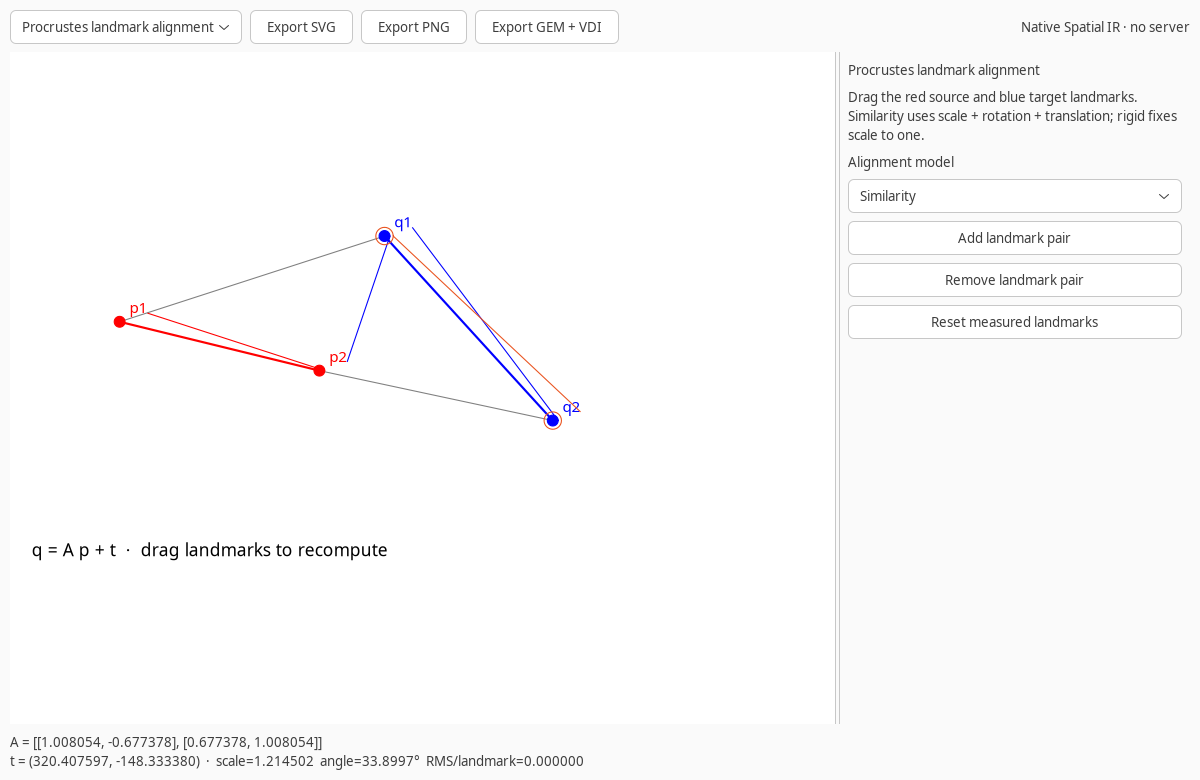
\includegraphics[width=\textwidth]{geometry-atlas.png}
\caption{Native Procrustes playground with draggable landmarks and live transform and residual inspection.}
\label{fig:geometry-atlas}
\end{figure}

\section{Dorothy and Neurogarden}
\subsection{Preclinical atlas geometry and memorial scope}
Dorothy is Zoe's spatial scientific-research priority: an inspectable workbench supporting a long-term brain-cancer research mission rather than a diagnostic or treatment system. The atlas is named in memorial for Dorothy McEwen Kildall; that dedication is not a source of patient anatomy. Its default geometry is the Allen Mouse CCFv3 2017 whole-brain parcellation \cite{wang2020allen}: 12 selected structures, 158,326 vertices, and 315,932 triangles, with source meshes and the structure graph hash-checked on every load.

The deterministic renderer supplies near-plane clipping, two-sided flat shading, painter-order display, and SVG/PNG/GEM VDI export. Dorothy Rings uses exact CCF subtree volumes for ontology drill-down; Jenga uses volume-scaled layers and exploded/pull-out layouts; Stack cuts actual meshes into exploded coronal slabs. These are alternative geometric views of the same preclinical reference data, not functional connectivity, patient registration, surgical planning, or a claim that mouse anatomy transfers to a person.

\begin{figure}[htbp]
\centering
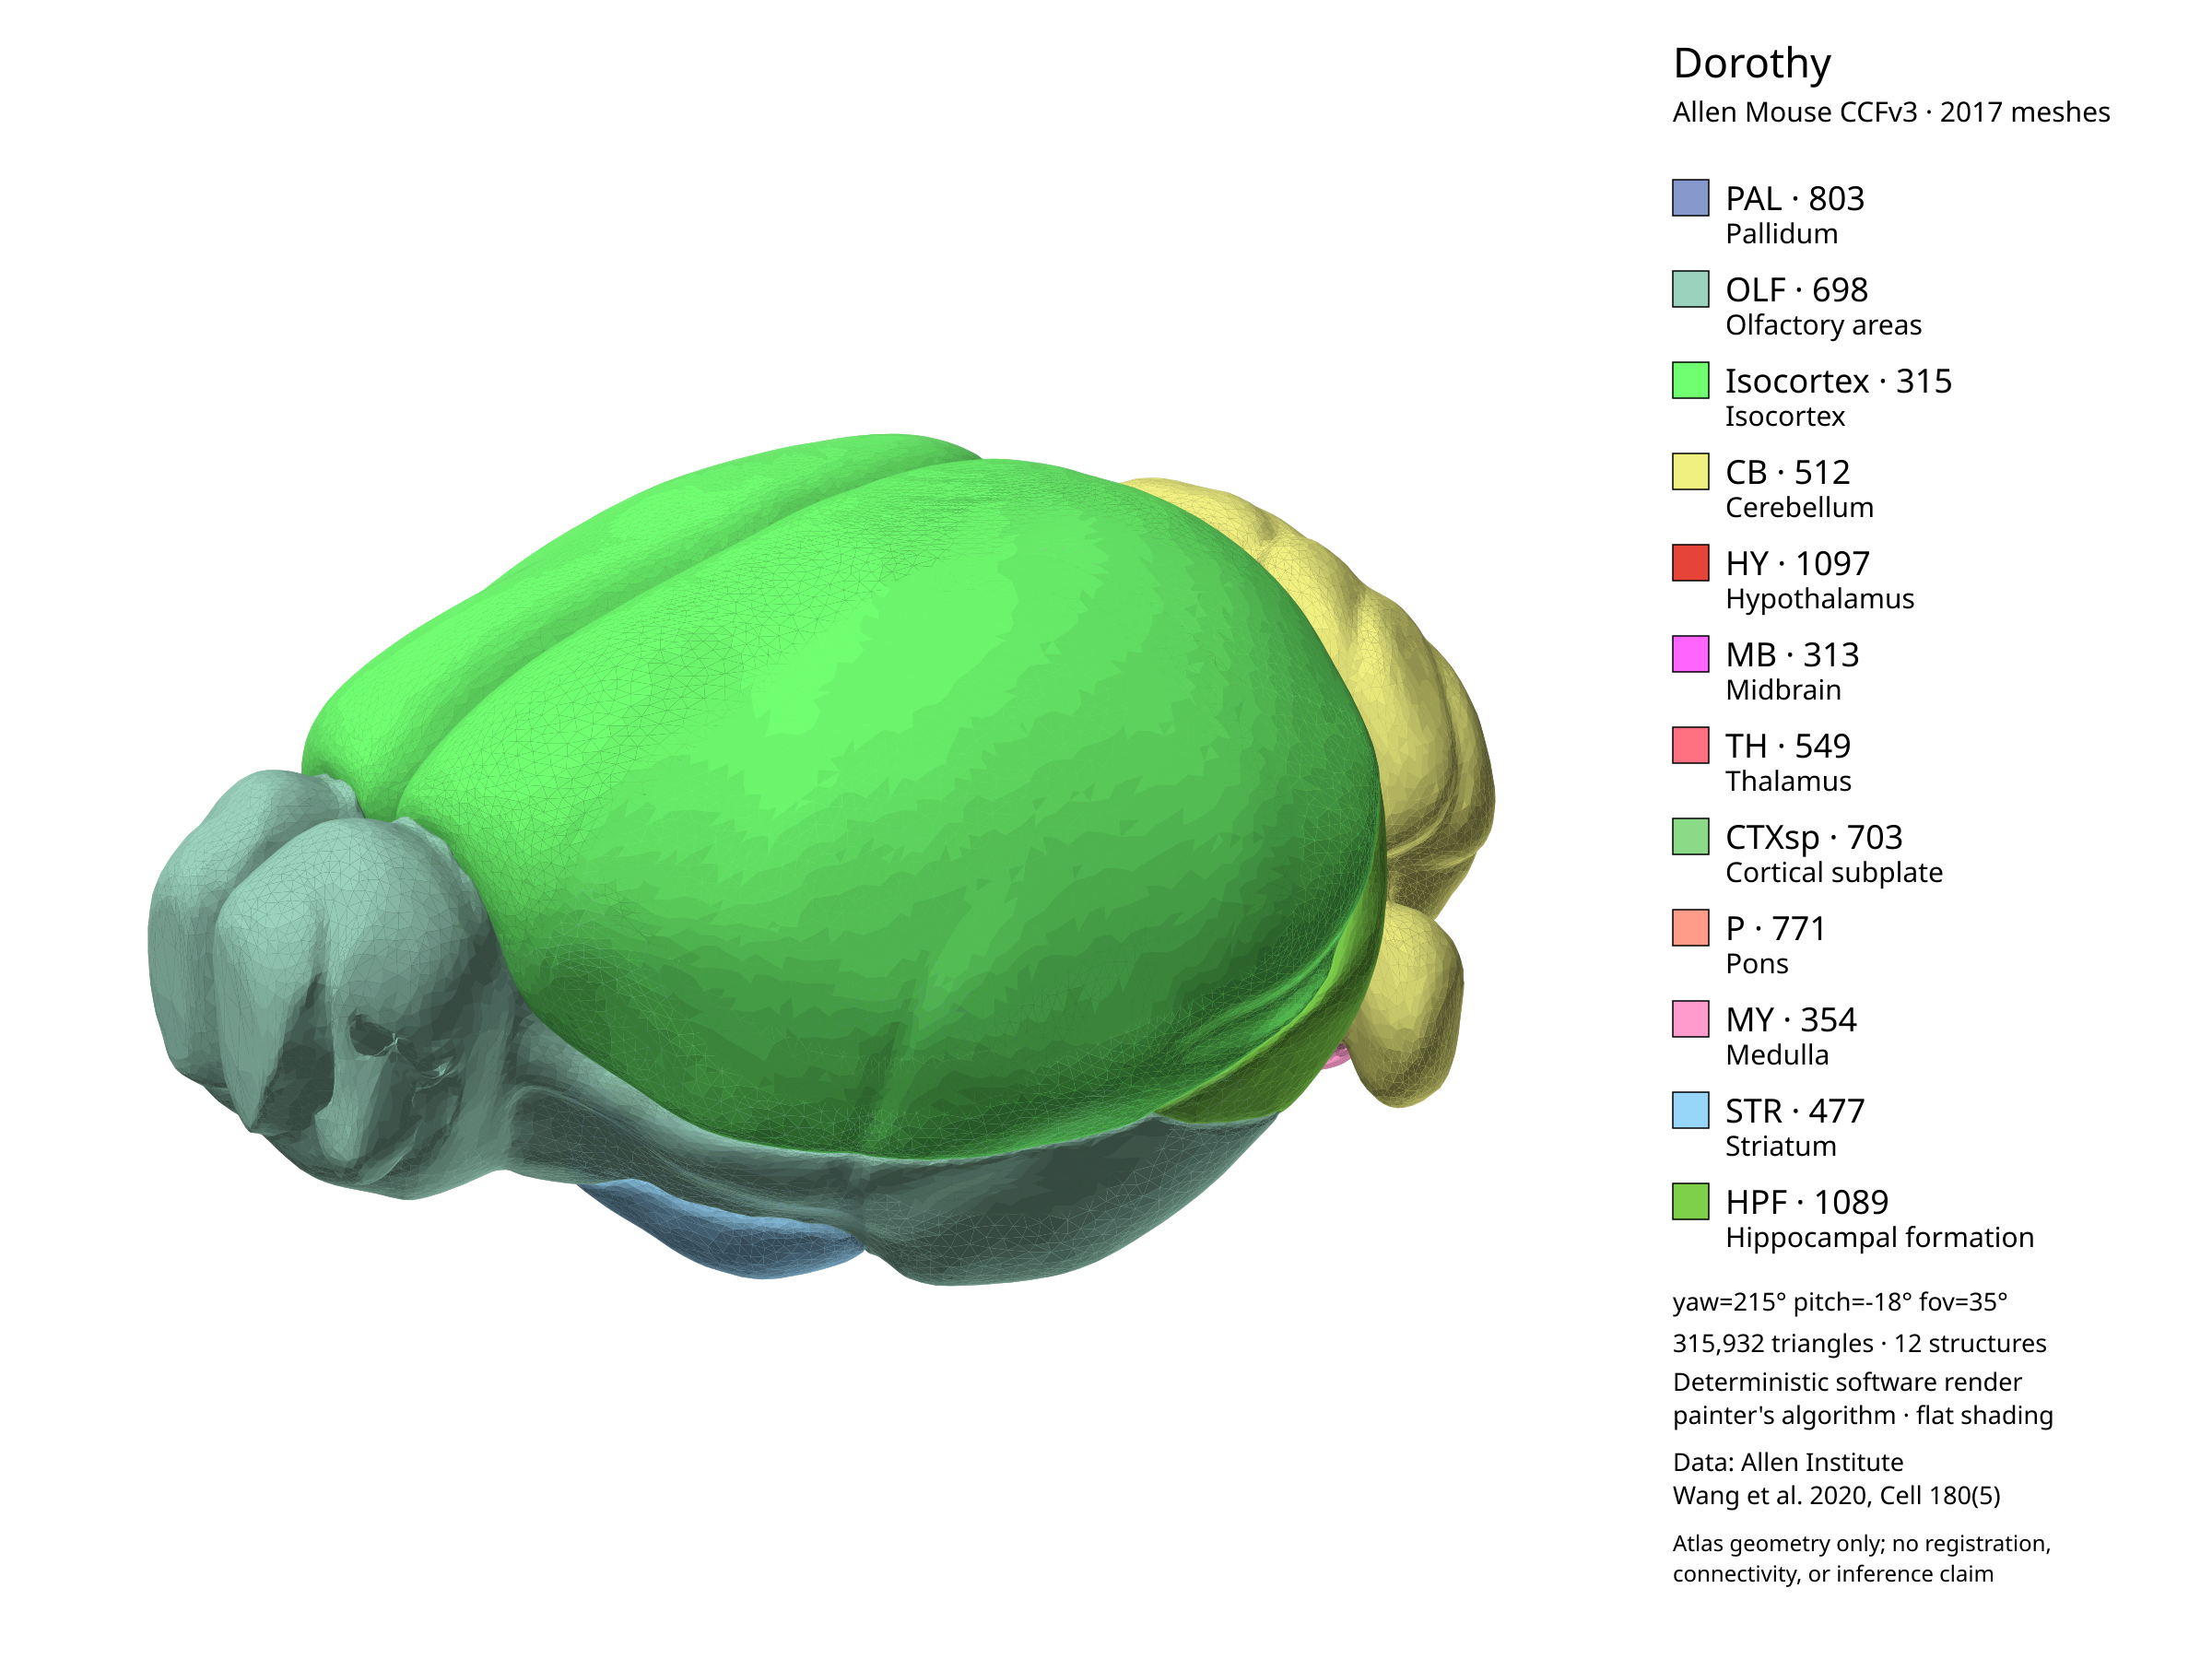
\includegraphics[width=\textwidth]{dorothy-ccf2017.png}
\caption{Dorothy's deterministic Allen Mouse CCFv3 atlas rendering. The twelve displayed structures are preclinical reference geometry, not patient imaging or diagnostic evidence.}
\label{fig:dorothy-atlas}
\end{figure}

\begin{figure}[htbp]
\centering
\begin{tabular}{@{}c@{}c@{}}
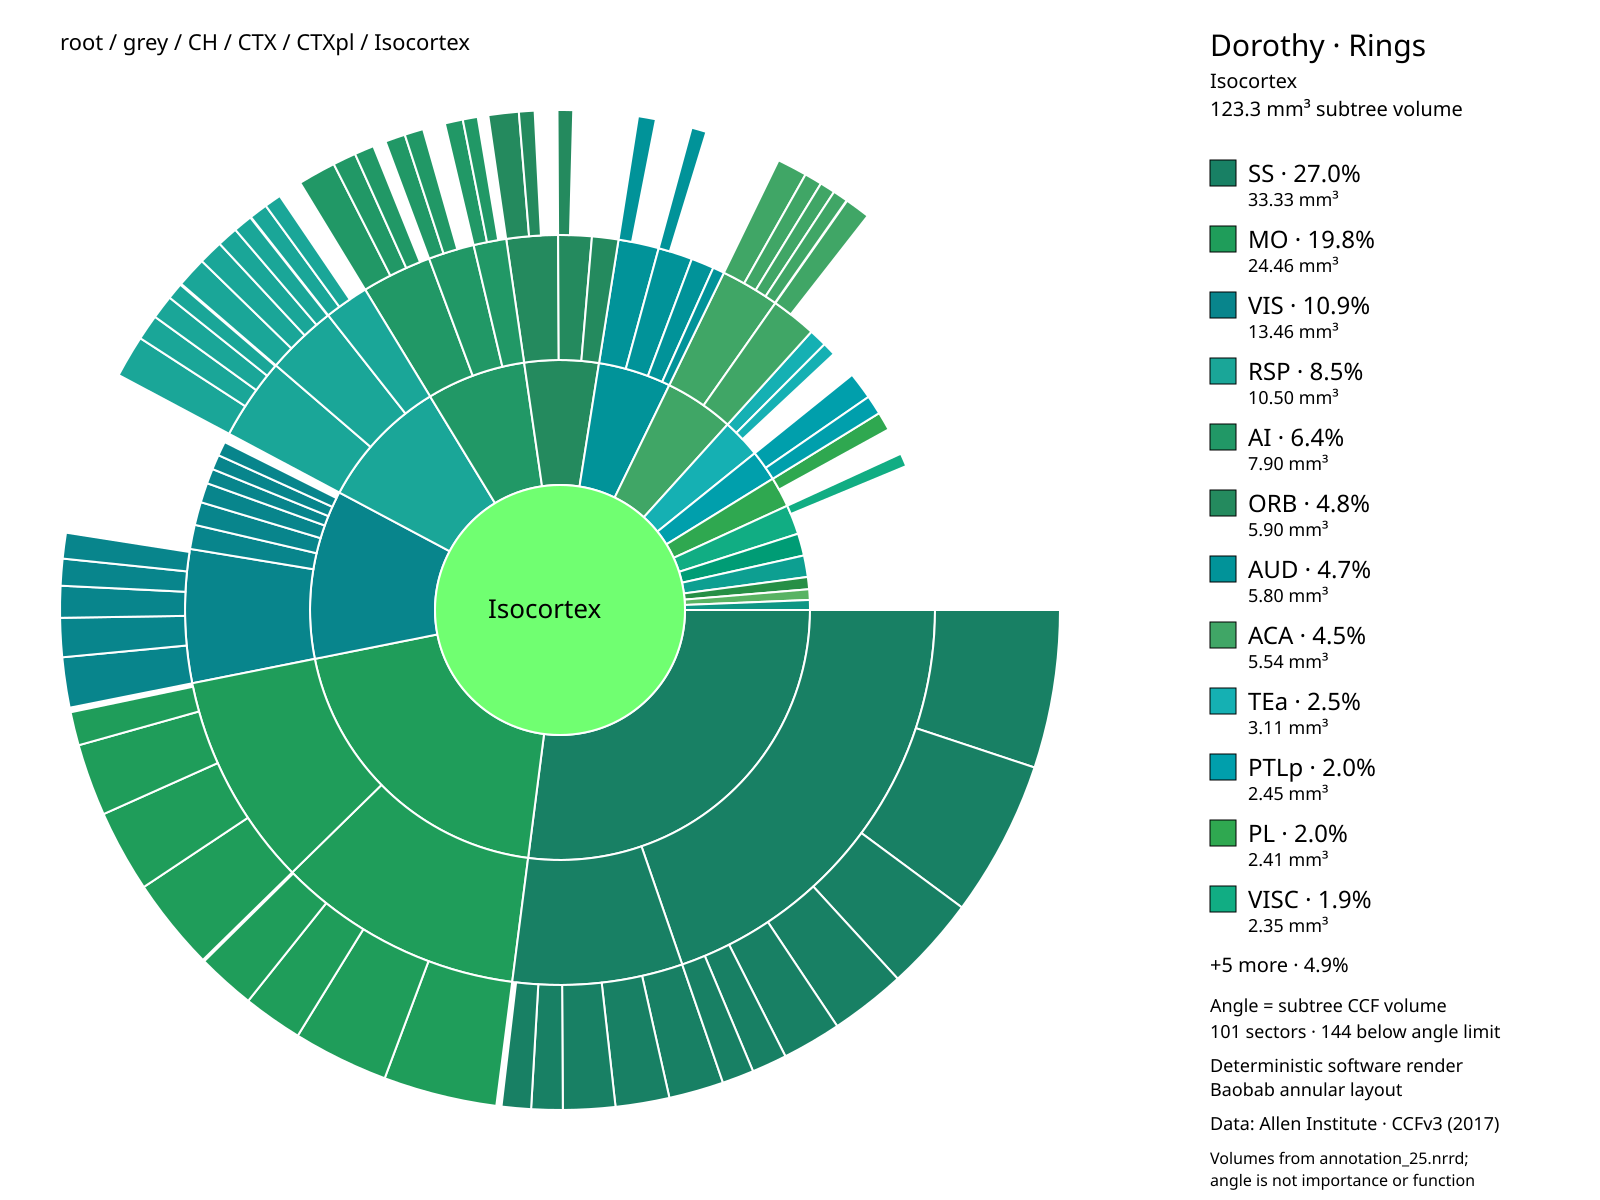
\includegraphics[width=0.48\textwidth]{dorothy-rings-isocortex.png}&
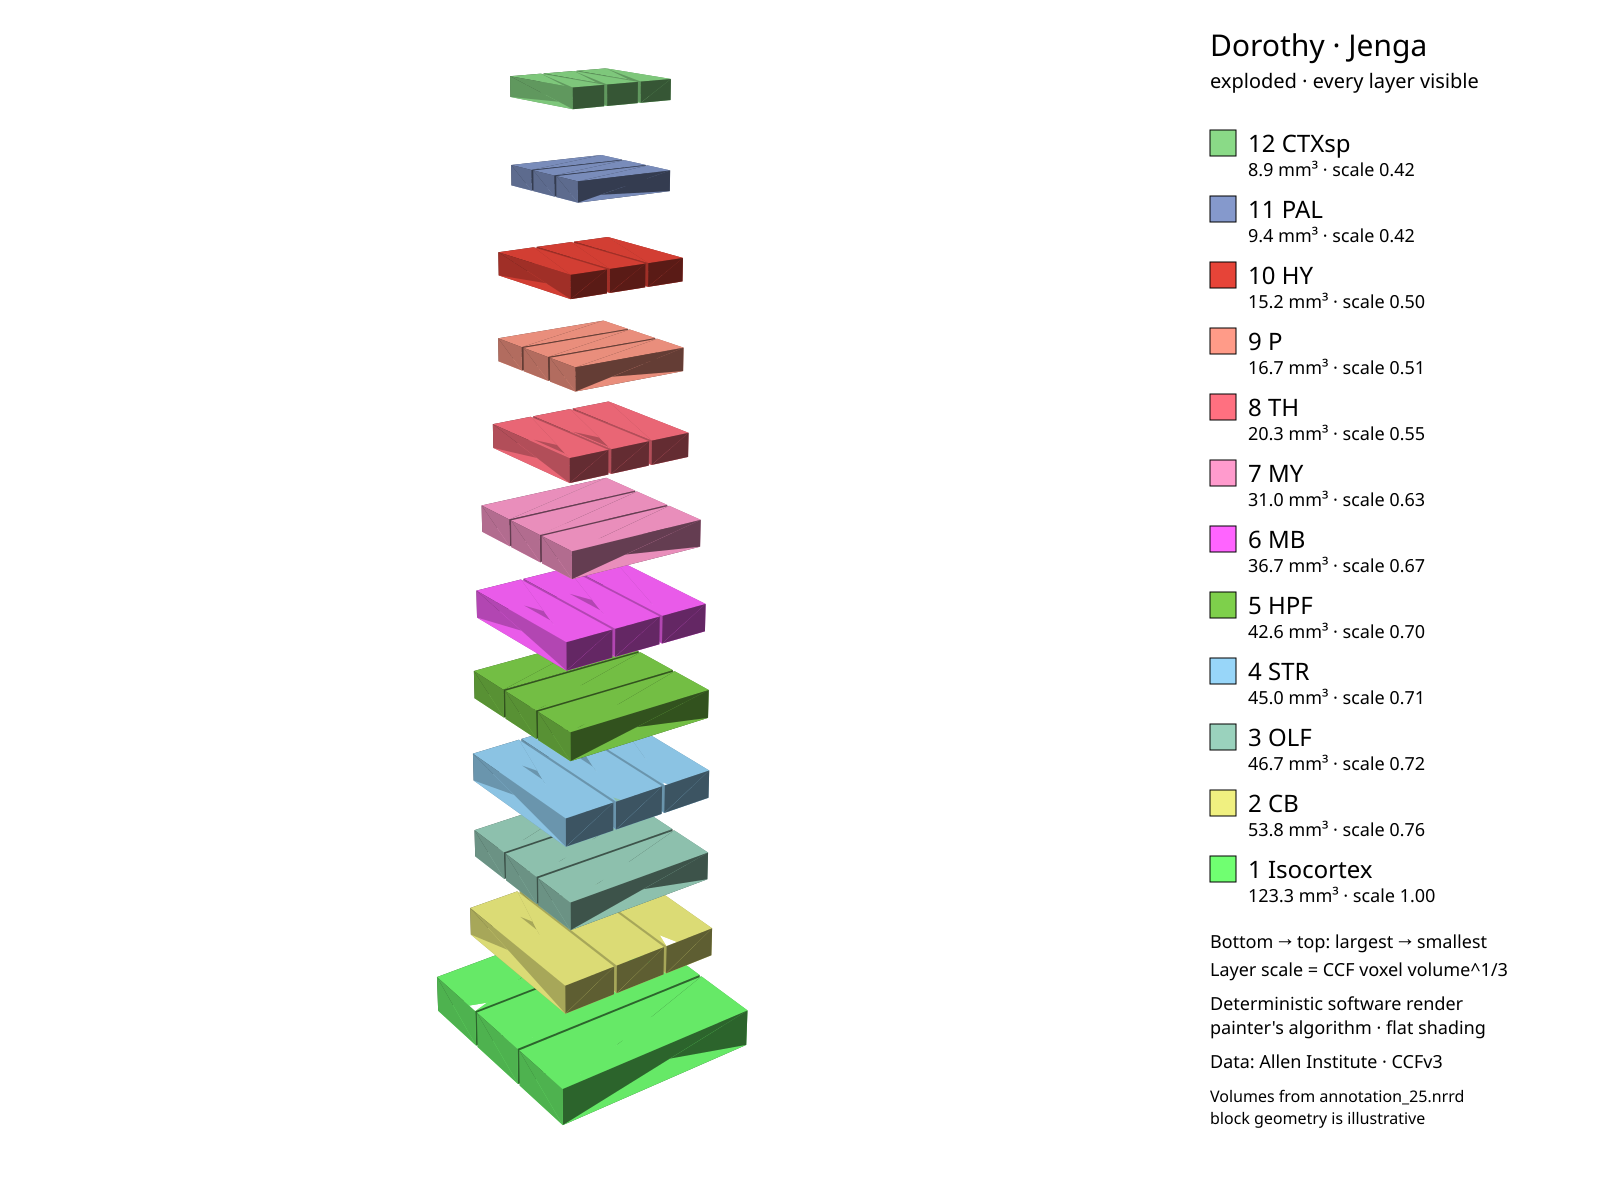
\includegraphics[width=0.48\textwidth]{dorothy-jenga-exploded.png}
\end{tabular}
\caption{Dorothy Rings and Jenga expose ontology volume and spatial layout without asserting functional or clinical relationships.}
\label{fig:dorothy-layouts}
\end{figure}

\subsection{Source-linked Neurogarden review}
Neurogarden connects Dorothy, agent oversight, synthetic teaching models, and a cited research library. Its review state distinguishes \texttt{cataloged}, \texttt{extracted}, and \texttt{reviewed}; extraction and keyword indexing are not comprehension. A review requires source hashes, concepts, applications, limitations, and either a demonstrated bounded use or an explicit no-tool rationale. Duplicate JSON keys and conflicting use/no-tool states are rejected. Clinical references enter human review and do not authorize action.

At the November 14 source state, the corpus contained 37 populated books, 1,751 indexed sections, 130 reviewed entries, and 1,621 pending entries. The current v62 evidence preserves source hashes and bounded snippets rather than republishing books. Sixty-two focused Neurogarden tests and three C99 legacy suites were recorded as passing; these verify the exercised software, not medical validity.

Representative teaching instruments include bounded Needleman--Wunsch global alignment. For match/mismatch score $s(a_i,b_j)$ and gap penalty $g$,
\begin{equation}
D_{i,j}=\max\begin{cases}
D_{i-1,j-1}+s(a_i,b_j),\\
D_{i-1,j}+g,\\
D_{i,j-1}+g,
\end{cases}
\end{equation}
with first row and column initialized by cumulative gap penalties. The implementation reproduces the reviewed example's score four and seven optimal paths while bounding sequence length and retained paths. An alignment score is not a species, identity, or clinical conclusion.

For imaging sampling, the educational ratio
\begin{equation}
N_{\mathrm{FWHM}}=\frac{\mathrm{FWHM}}{\Delta x}
\end{equation}
compares point-spread-function width with voxel spacing; finer sampling cannot create detail the imaging system did not capture. For a linear shift-invariant Gaussian teaching model, the modulation transfer function is
\begin{equation}
\operatorname{MTF}(k)=e^{-2\pi^2\sigma^2k^2},
\end{equation}
showing high-frequency suppression under blur without supplying scanner calibration. The spatial bench uses synthetic volumes up to $16^3$ voxels, separable Gaussian convolution, projections, pooling, and recovery coefficients. It does not register Dorothy to a patient.

\begin{figure}[htbp]
\centering
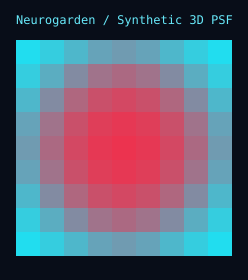
\includegraphics[width=\textwidth]{neurogarden-spatial.png}
\caption{Neurogarden's synthetic point-spread and projection bench. The image is an educational numerical scene, not anatomical or clinical data.}
\label{fig:neurogarden-spatial}
\end{figure}

The research record also preserves negative and contradictory source findings: incorrect specificity denominators, inconsistent MRI figure/table counts, swapped retinal plots, undefined SSIM scales, incomplete optimizer equations, missing patient-level splits, and unavailable raw predictions. Bounded arithmetic audits check printed values without training a model or converting secondary claims into clinical evidence. The complete current corpus index, reviews, and focused audits are included in the research collection.

Dorothy therefore extends Zoe's autonomy theme in a deliberately limited direction: a system can inspect geometry, preserve provenance, and propose research without acquiring diagnostic authority. Measurement remains distinct from evidence, belief, and action.

\section{Why the extended instruments matter}
These modules demonstrate a reusable research discipline: define the probability or state space, expose the equation, bound enumeration, preserve negative results, separate observation from authorization, and replay state transitions. Tetris supplies a nontrivial exact multi-horizon distribution; Pentacube supplies reversible transition arithmetic; the Internal Clock supplies state-responsive but non-autonomous timing; Halo preserves a failed spectral baseline; stereo and projection expose approximation error; EKF makes dynamics an external assumption. They are therefore methodological context for Zoe Autonomy, not additional dimensions in its full-autonomy predicate.
